\documentclass[11pt]{article}
\usepackage{fullpage}
\usepackage{amsmath,amsfonts,amsthm,amssymb}
\usepackage{url}
\usepackage{graphicx}
\usepackage{caption} 
\usepackage{algpseudocode}
\usepackage{bbm}
\usepackage{float}
\usepackage{framed}
\usepackage{enumerate}
\usepackage{color}
\usepackage[colorlinks=true, linkcolor=red, urlcolor=blue, citecolor=blue]{hyperref}
\usepackage{listings}

\DeclareMathOperator*{\E}{\mathbb{E}}
\let\Pr\relax
\DeclareMathOperator*{\Pr}{\mathbb{P}}
\DeclareMathOperator*{\R}{\mathbb{R}}
\DeclareMathOperator*{\Var}{\textrm{Var}}

\topmargin 0pt
\advance \topmargin by -\headheight
\advance \topmargin by -\headsep
\textheight 8.9in
\oddsidemargin 0pt
\evensidemargin \oddsidemargin
\marginparwidth 0.5in
\textwidth 6.5in

\parindent 0in
\parskip 1.5ex

\newcommand{\homework}[2]{
	\noindent
	\begin{center}
		\framebox{
			\vbox{
				\hbox to 6.50in { {\bf NYU CS-GY 9223D: Algorithmic Machine Learning 
						and Data Science} \hfill Fall 2020 }
				\vspace{4mm}
				\hbox to 6.50in { {\Large \hfill Homework #1  \hfill} }
				\vspace{2mm}
				\hbox to 6.50in { {Name: #2 \hfill} }
			}
		}
	\end{center}
	\vspace*{4mm}
}

\newcommand{\braket}[2]{\langle #1, #2\rangle}
\newcommand{\norm}[1]{||#1||_2}

\begin{document}
	
%\homework{1}{R. Teal Witter}
%\section*{Problem 1}
\textbf{Collaborators:} Avery Anderson.
\medskip

\begin{enumerate}
    \item Fix $k > 0.$ Now define the random variable $X$ in the following way:
    $X$ takes value $\sqrt{10}k$ with probability $1/20k^2$,
    $-\sqrt{10}k$ with probability $1/20k^2$,
    and 0 with probability $1-1/10k^2$.
    Then
    \begin{align}
        \E[X] = \sqrt{10}k \times \frac{1}{20k^2} - \sqrt{10}k \times \frac{1}{20k^2}
        + 0 \times (1 - \frac{1}{10k^2}) = 0
        \nonumber
    \end{align}
    and
    \begin{align}
        \E[X^2] = (\sqrt{10}k)^2 \times \frac{1}{20k^2} +
        (-\sqrt{10}k)^2 \times \frac{1}{20k^2}
        + 0^2 \times (1 - \frac{1}{10k^2}) = 1.
        \nonumber
    \end{align}
    It follows that the variance of $X$ $\sigma^2$ is
    $\E[X^2] - \E[X]^2 = 1 - 0^2 = 1$.
    Now Chebyshev's Inequality says that 
    \begin{align}
        \Pr(|X-\E[X]| \geq k \sigma) \leq \frac{1}{k^2}
        \nonumber
    \end{align}
    and, in this case, 
    \begin{align}
        \Pr(|X| \geq k) \leq \frac{1}{k^2}.
        \nonumber
    \end{align}
    By inspection of $X$, we know that $|X| \geq k$
    only when $X=k$ or $X=-k$ so
    \begin{align}
        \Pr(|X| \geq k) = \frac{1}{10k^2}.
        \nonumber
    \end{align}
    We have equality up to a constant factor.
    \qedsymbol
    
    \item The probability that we do not see heads in $n$
    flips is $(1 -1/n)^n$. Then
    \begin{align}
        (1-\frac{1}{n})^n \leq
        \lim_{n \rightarrow \infty} (1 -\frac{1}{n})^n = e^{-1} \approx 
        .3679.
        \nonumber
    \end{align}
    The inequality holds because we are approaching the limit from
    the left. (Checking progressively larger values of $n$ makes this apparent.)
    
    Now let's repeat our $n$ flips $\log n$ times.
    The probability that a head does not appear in $n$ flips $\log n$
    times is $(1-1/n)^{n \log n}$.
    It follows from $(1-1/n) \leq e^{-1}$ that
    \begin{align}
        \left((1-\frac{1}{n})^n)\right)^{\log n} \leq
        (e^{-1})^{\log n} = (e^{\log n})^{-1} = \frac{1}{n}
        \nonumber
    \end{align}
    since $x^{\log n}$ is a monotone increasing function for $n > 1$.
    \qedsymbol
    
    \item The probability that we have no collision is
    \begin{align}
        1 \times (1 - \frac{1}{m^2}) \times (1 - \frac{2}{m^2}) \times
        \dots \times (1 - \frac{m-1}{m^2}).
        \nonumber
    \end{align}
    The Taylor series expansion of $e^x$ is $1+x$ for $|x| << 1.$
    Then $1-i/m^2 = e^{-i/m^2}$.
    Plugging back in, we have
    \begin{align}
        &\approx 1 \times e^{-1/m^2} \times e^{-2/m^2} \times
        \dots \times e^{-(m-1)/m^2} \nonumber \\
        &= e^{-(1+2+\dots+m-1)/m^2} = e^{-m(m-1)/2m^2} \nonumber \\
        &= e^{-1/2 (1 - 1/m^2)} =
        \left(\frac{e}{e^{1/m^2}}\right)^{-1/2} \nonumber \\
        &= \sqrt{\frac{e^{1/m^2}}{e}} \leq .6873
        \nonumber
    \end{align}
    for $m>1$.
    We see that the inequality holds since the expression decreases
    as $m$ increases with a lower bound of $\sqrt{1/e} \approx .6065$.
    \qedsymbol
    
    \item We want to bound the probability that any event $A_i$
    occurs for $1 \leq i \leq k$.
    Let $X_i$ be the indicator random variable that takes value 1
    if $A_i$ occurs and 0 otherwise.
    Then
    \begin{align}
        \label{eq:unionmarkov}
        \Pr(A_1 \cup A_2 \cup \dots \cup A_k) &=
        \Pr(X_1 + X_2 + \dots + X_k \geq 1) \\
        \label{eq:unionlinear}
        & \leq \frac{\E[X_1+X_2 + \dots X_k]}{1}\\
        \label{eq:unionindicator}
        &= \sum_{i=1}^k \E[X_i] = \sum_{i=1}^k \Pr[A_i] 
    \end{align}
    where \autoref{eq:unionlinear} follows from
    \autoref{eq:unionmarkov} by Markov's Inequality and
    \autoref{eq:unionindicator} follows from 
    \autoref{eq:unionlinear} by the Linearity of Expectation.
    The equality in \autoref{eq:unionindicator} follows
    from the following property of indicator random variables:
    \begin{align}
        \E[X_i] = 0 \times (1-\Pr(A_i)) + 1 \times \Pr(A_i) =
        \Pr(A_i).
        \nonumber
    \end{align}
    \qedsymbol
    
\end{enumerate}
    
\newpage
\section*{Problem 2}
\textbf{Collaborators:}  None.
\medskip

\begin{enumerate}
    \item We want to build a random variable that counts the
    number of collisions in our hashing scheme.
    Let $X_{i,j,k}$ be the indicator random variable that takes
    value 1 if and only if the $i$, $j$, and $k$ hashed items are all 
    the same for $i,j,k \in [m]$ and $i\neq j \neq k \neq i$.
    Then $X$ is the sum of $X_{i,j,k}$.
    We take the expectation
    \begin{align}
        \E[X] &= \binom{m}{3} \Pr(X_{i,j,k}=1) =
        \frac{m(m-1)(m-2)}{3!} \frac{1}{m^{1.5}m^{1.5}} \nonumber \\
        &= \frac{m^3 -3m^2 + 2m}{6m^3} \leq \frac{1}{6}
        \nonumber
    \end{align}
    for $m > 1$.
    Using Markov's Inequality, the probability that we have at least
    one collision is
    \begin{align}
        \Pr(X \geq 1) \leq \frac{E[X]}{1} \leq \frac{1}{6} \nonumber.
    \end{align}
    \qedsymbol
    
    \begin{figure}[H]
        \centering
        \fbox{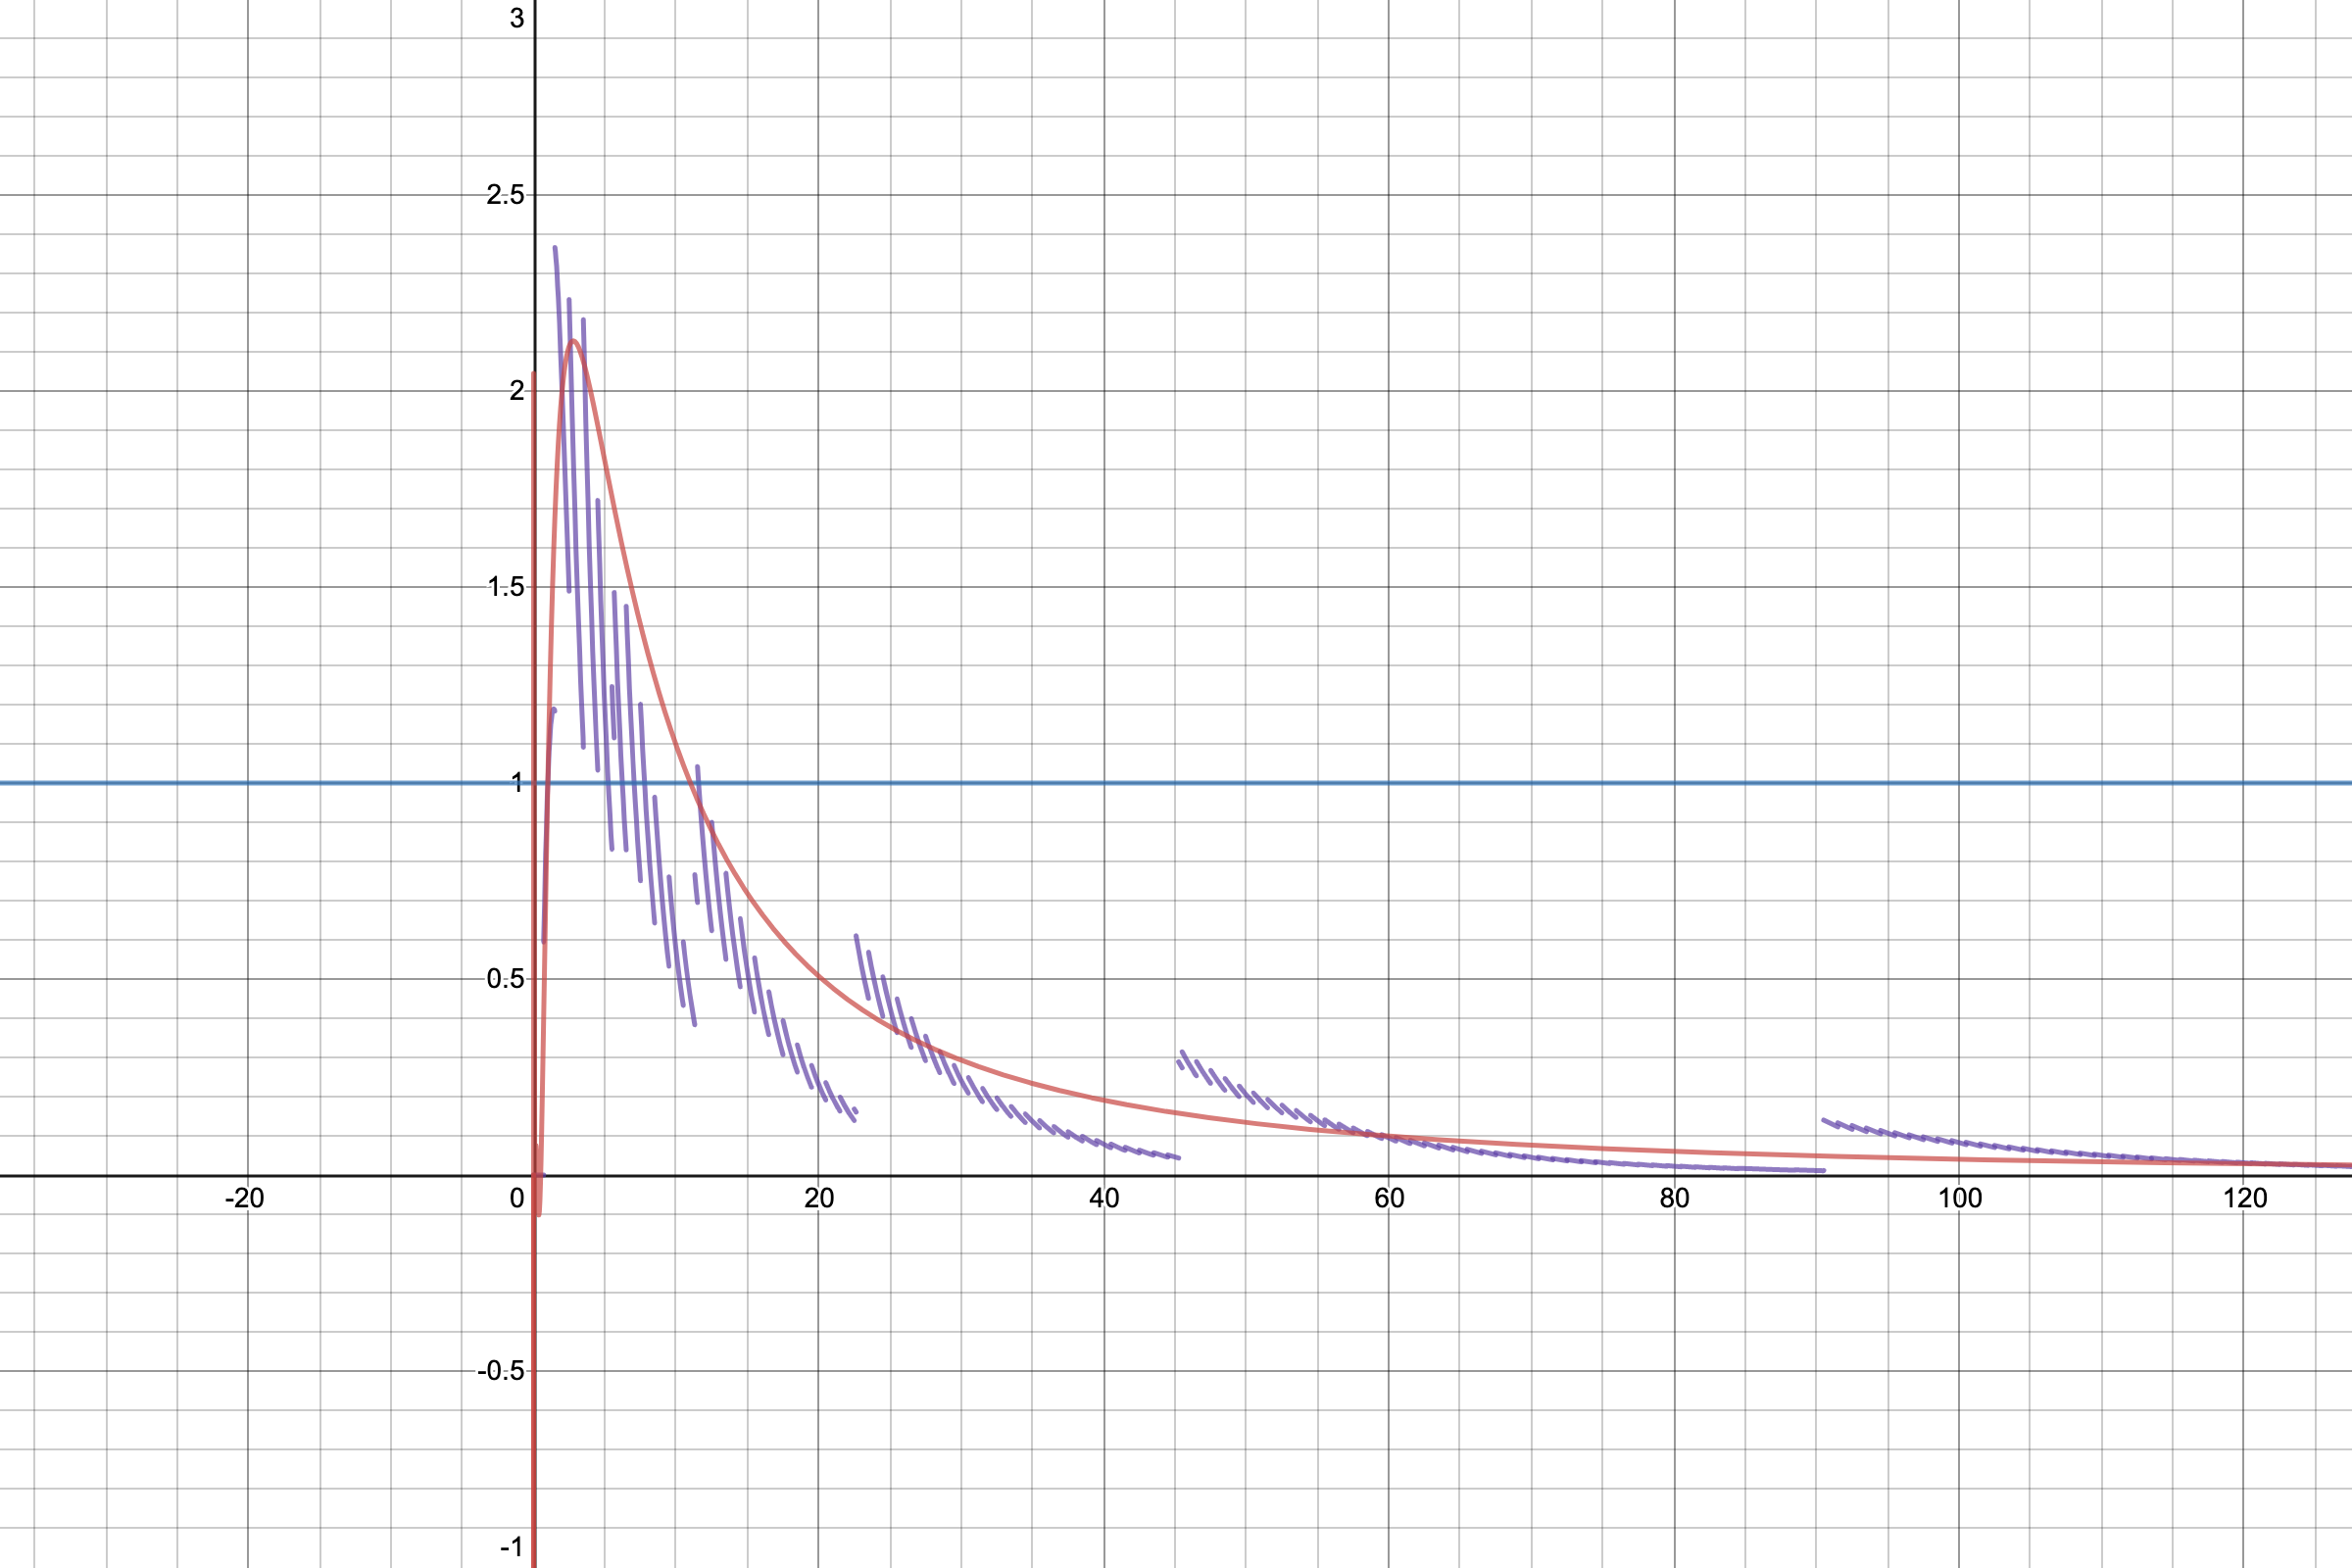
\includegraphics[scale=.2]{graphics/1.2.2.png}}
        \caption{The blue line is $y=1$, the purple line is
        $y=\binom{m}{\log_2 m}/m^{\log_2 m -1}$, and the red line
        is $y = m/(\log_2 m)!$.
        For sufficiently large $m$, the red line and purple lines
        get arbitrarily small.
        The original Desmos plot may be viewed 
        \href{https://www.desmos.com/calculator/64kvnqp8ho}{here}.}
        \label{fig:1.2.2}
    \end{figure}
    
    \item We will take the same approach.
    Define $n = \log_2 m$.
    Let $X_i$ be the indicator random variable that takes value
    1 if and only if all $n$ values of subset $i$ of $[m]$ are all hashed
    to the same value.
    We take the expectation
    \begin{align}
        \E[X] &= \binom{m}{n} \Pr(X_i) \nonumber \\
        &= \frac{m(m-1)(m-1)\dots(m-n+1)}{n!} \frac{1}{m^{n-1}} \nonumber \\
        & \approx \frac{m}{(\log_2 m)!}.
        \nonumber
    \end{align}
    \autoref{fig:1.2.2} shows how $\E[X]$ gets arbitrarily small
    as $m$ increases.
    It follows from Markov's Inequality that, for sufficiently large $m$,
    there is a very low probability of collisions with
    $\log m$ hash tables all of size $O(m)$.
    \qedsymbol
\end{enumerate}   



\newpage
\section*{Problem 3}
\textbf{Collaborators:}  Indu Ramesh.
\medskip

\begin{enumerate}
    \item Set $k=5/\epsilon^2$.
    Define indicator random variable $Y_i$
    that takes value 1 if and only if $X_i$
    comes from the smallest $1/2-\epsilon$
    fraction of $S$.
    Then
    $\E[Y_i] = \E[Y_i^2] =\Pr(Y_i=1) = 1/2-\epsilon$
    by the properties of indicator random variables.
    We now calculate the variance
    \begin{align}
        \Var(Y_i) &= \E[Y_i^2] - \E[Y_i]^2 \nonumber \\
        &=\frac{2-4\epsilon}{4} -
        \frac{1-2\epsilon + \epsilon^2}{4} \nonumber \\
        &= \frac{1-2\epsilon-\epsilon^2}{4}.
        \nonumber
    \end{align}
    Let $Y$ be the sum of $Y_i$.
    By linearity of expectation, $\E[Y] = k/2-k\epsilon$.
    Since the $X_i$ are drawn with replacement,
    the $Y_i$ are independent.
    By linearity of variance for independent variables,
    $\Var(Y) = k(1-2\epsilon-\epsilon^2)/4$.
    
    Observe that $1/2-\epsilon$ of the numbers in $S$
    are less than $\bar{M}$ if and only if the number
    of $X_i$ that come from the smallest $1/2-\epsilon$
    fraction of $S$ is greater than $k/2$.
    Therefore we want to bound
    using Chebyshev's inequality
    \begin{align}
        \Pr(Y > \frac{k}{2}) &=
        \Pr(Y > \frac{k}{2} -k \epsilon + k \epsilon)
        \nonumber \\
        &= \Pr(Y - \left(\frac{k}{2}-k\epsilon\right)>k\epsilon)
        \nonumber \\
        &\leq \Pr(|Y - \E[Y]| \geq k\epsilon)
        \nonumber \\
        &\leq \frac{\Var(Y)}{(k\epsilon)^2} =
        \frac{k-2k\epsilon -k\epsilon^2}{4}\frac{1}{k^2\epsilon^2}
        \nonumber \\
        &< \frac{1}{4k\epsilon^2}
        = \frac{1}{20}
        \nonumber
    \end{align}
    since $k=5/\epsilon^2$ and $\epsilon>0$.
    By symmetry, the probability that more than
    $k/2$ $X_i$ come from the largest $1/2+\epsilon$
    fraction of $S$ is also less than $1/20$.
    Then with probability $9/10$ at least
    $1/2-\epsilon$ numbers in $S$ are smaller
    than $\bar{M}$ and at least 
    $1/2+\epsilon$ numbers in $S$ are larger.
    \qedsymbol
    
    \begin{figure}[H]
        \centering
        \fbox{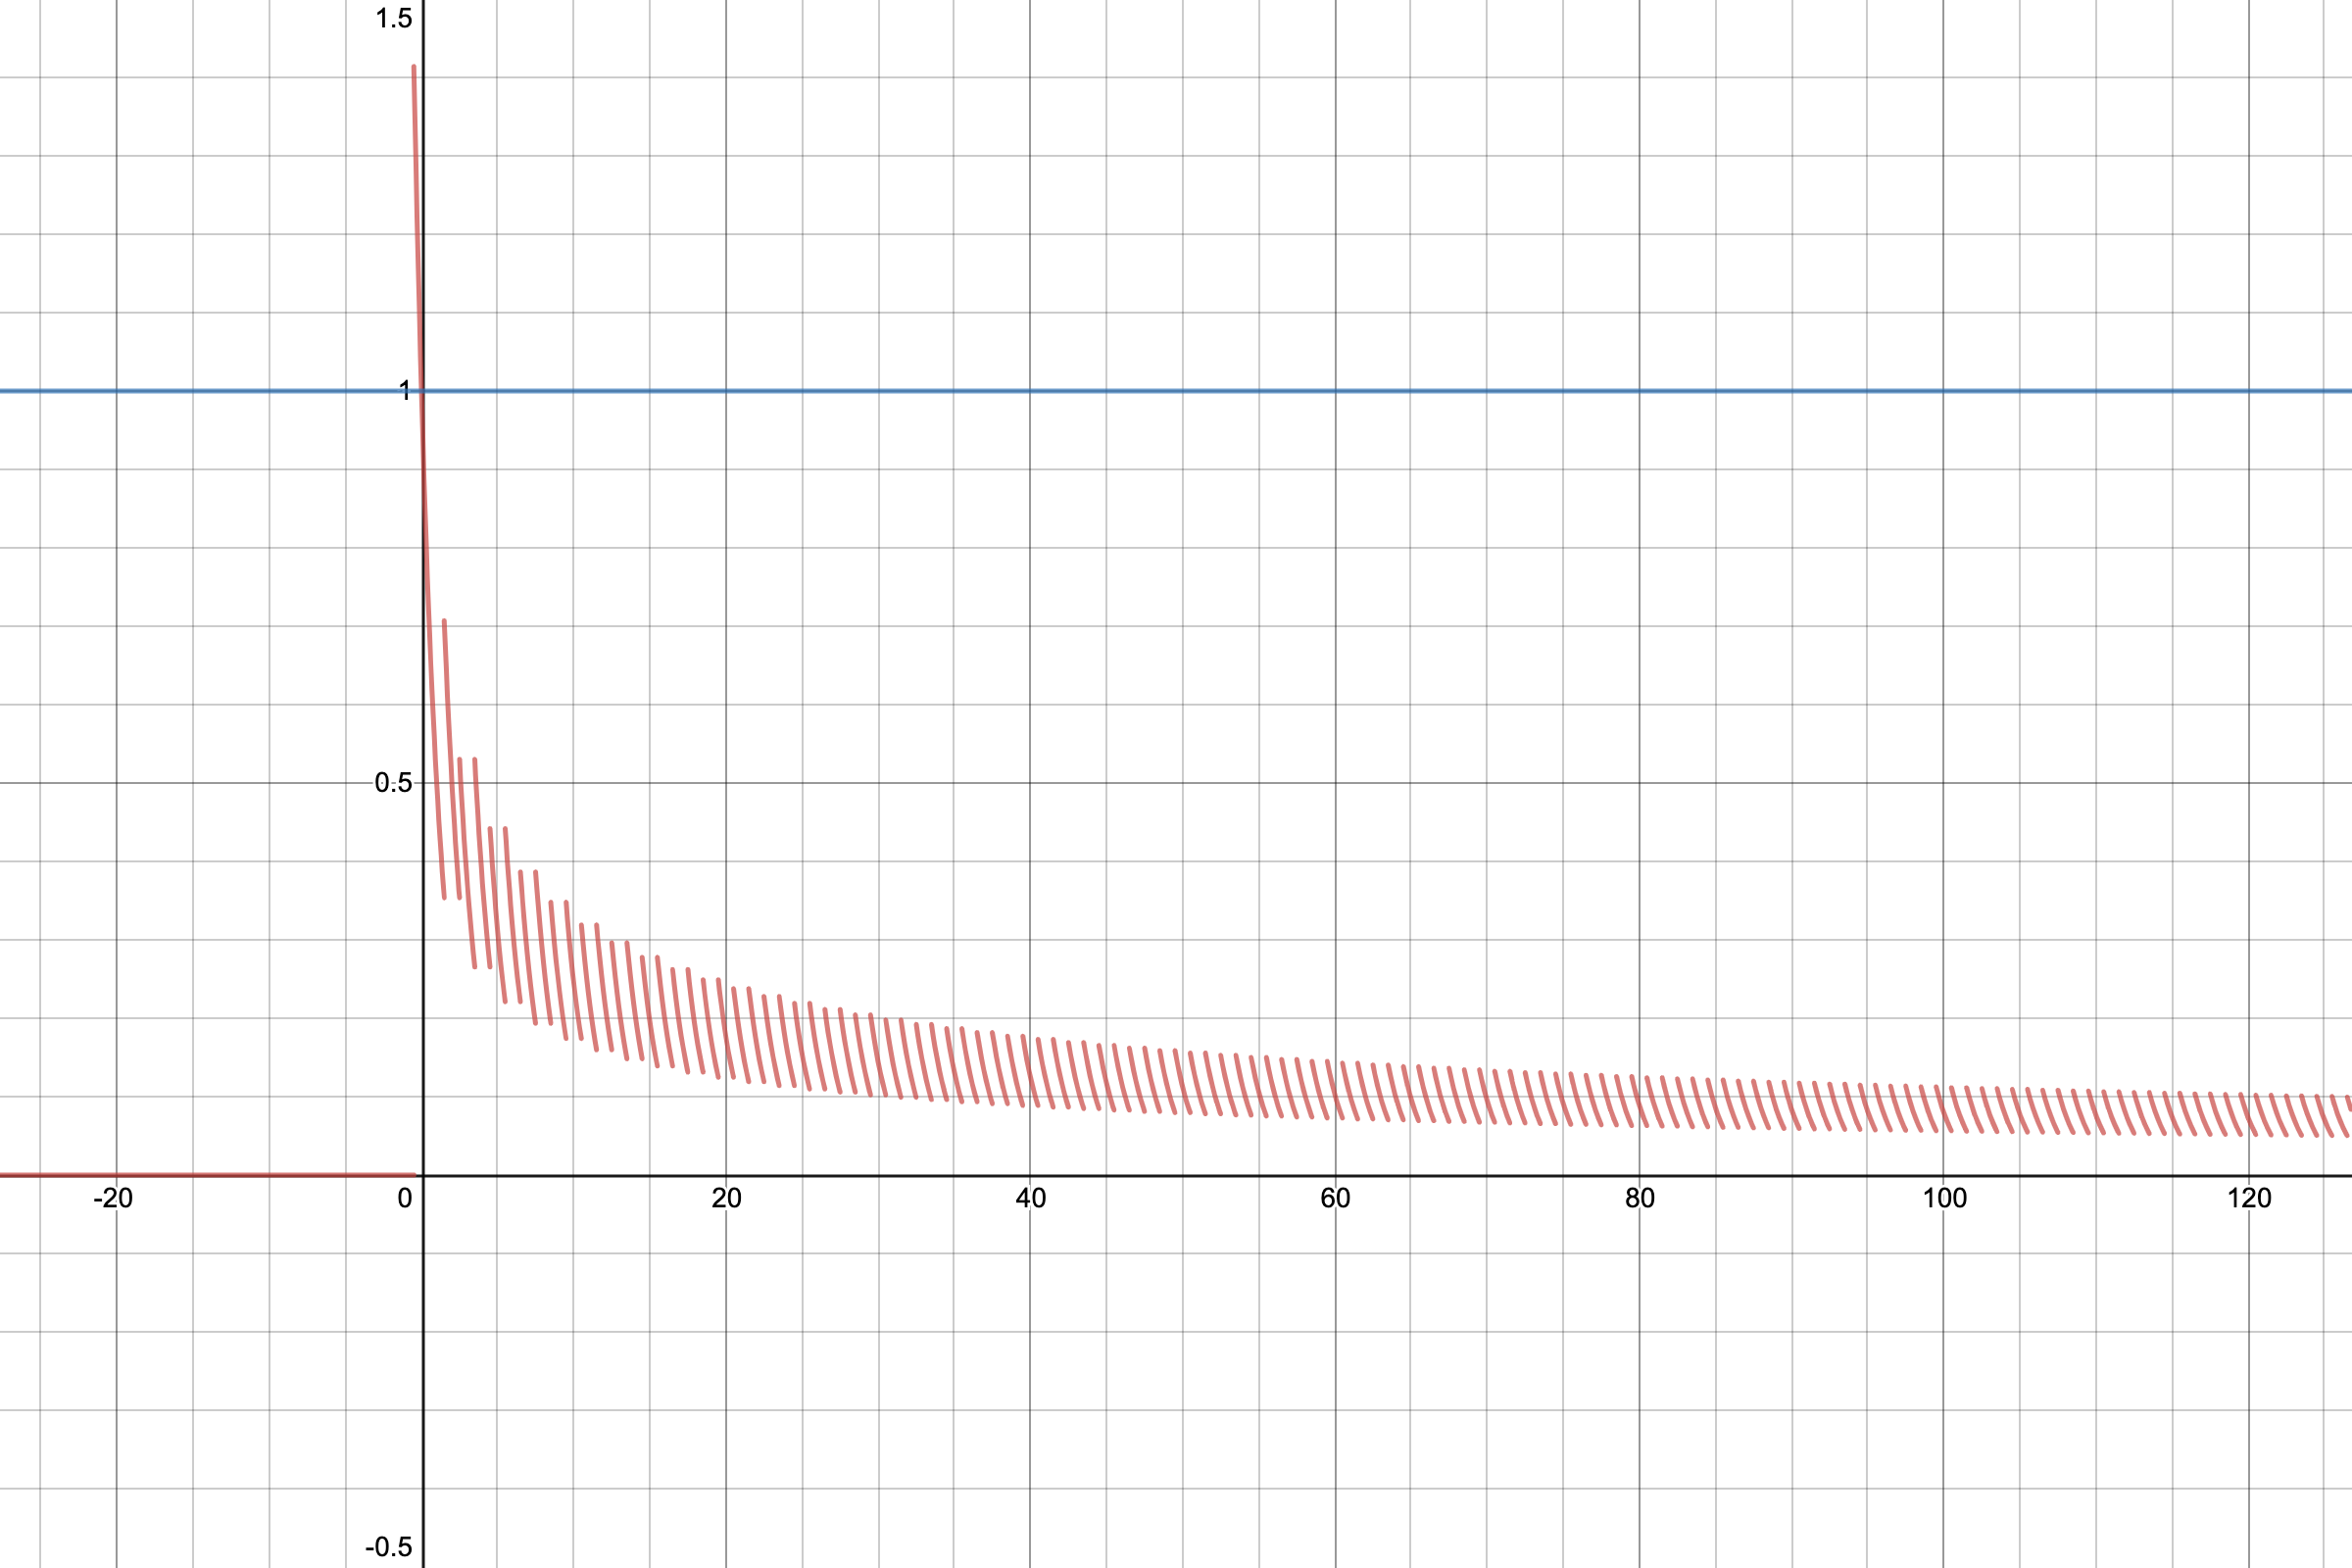
\includegraphics[scale=.2]{graphics/1.3.2.png}}
        \caption{The blue line is $y=1$, and the red line
        is $y = \binom{k}{k/2}1/2^k$.
        For $k>1$, the red line is less than 1 and decreasing.
        The original Desmos plot may be viewed 
        \href{https://www.desmos.com/calculator/zaeb2c8qvf}
        {here}.}
        \label{fig:1.3.2}
    \end{figure}
    
    \item We construct an adversarial $S$
    to show that $o(n)$ samples are not sufficient
    to estimate $M$ within a multiplicative factor
    by $\bar{M}$.
    Let $n$ be even and $S$ a dataset consisting of
    -2 repeated $n/2$ times and 3 repeated $n/2$ times.
    The true median $M$ is 1.
    In a sample of size $k$ when $k$ is odd
    we will only ever have $\bar{M}$ equal to -2 and 3.
    Since neither value is between .5 and 2,
    $k$ must be even for us to have a chance to estimate $M$.
    If the two middle numbers in the sample $X_1,\dots,X_k$
    are -2, we fail.
    If the two middle numbers in the sample are 3,
    we also fail.
    If the two middle numbers in the sample are -2 and 3,
    we succeed.
    So the only way to estimate $M$ within our interval
    is if the sample has exactly as many -2's as 3's.
    The probability of this event is
    \begin{align}
        \binom{k}{k/2} \frac{1}{2}^{k/2} \frac{1}{2}^{k/2}
        = \binom{k}{k/2} \frac{1}{2}^k.
    \nonumber 
    \end{align}
    
    \autoref{fig:1.3.2} demonstrates how this probability
    decreases as $k$ grows.
    So, in fact, the probability of correctly estimating
    $M$ with $\bar{M}$ becomes increasingly unlikely
    for increasing $k$ and any $n$.
    \qedsymbol
    
\end{enumerate}

\newpage
\section*{Problem 4}
\textbf{Collaborators:}  None.
\medskip

\begin{enumerate}
    \item Let $C=\sqrt{nk}$.
    There are two rounds of tests: In the first round,
    we test each group for a total of $\sqrt{nk}$ tests.
    In the second round, we test each group that had a
    positive result. There are $n/\sqrt{nk} = \sqrt{n/k}$
    individuals in a group. In the worst case, each
    individual that is actually positive is in their own group
    so that's a total of $\sqrt{n/k}k = \sqrt{nk}$ more tests.
    Therefore we can identify all positive individuals
    with $2\sqrt{nk}$ tests or fewer.
    \qedsymbol
    
    \item Let $q=\log_2 n$ and $C=4k$.
    Define $A_i$ as the event that COVID-positive
    individual $i$ is in a particular group.
    Since the groups are drawn randomly,
    $P(A_i) = 1/C = 1/4k$.
    Then $P(A_1 \cup \dots \cup A_k) \leq k/4k =1/4$
    by the Union Bound.
    Let $X_i$ be the indicator random variable that COVID-negative
    individual $i$ is in $\log_2 n$ groups that \textit{all}
    test positive for $1 \leq i \leq n$.
    The probability that $X_i=1$ is less than or equal to
    $(1/4)^{\log_2 n}$.
    Now define the total number of false positives
    $X$ as the sum of $X_i$.
    Taking expectation since each event is independent,
    \begin{align}
        \E[X] &= (n-k) \Pr(X_i = 1) \nonumber \\
        &\leq (n-k) (2^{-2})^{\log_2 n} \nonumber \\
        &= \frac{n-k}{n^2} \leq 1/n.
        \nonumber
    \end{align}
    Markov's Inequality yields
    $\Pr(X\geq1) \leq 1/n$.
    Therefore we identify all actual positives and, 
    for $n>10$, we give no false positives with probability
    more than $9/10$.
    \qedsymbol
\end{enumerate}


%\homework{2}{R. Teal Witter}
%% chktex-file 46
% chktex-file 3

\section*{Problem 1}
\textbf{Collaborators:} Indu Ramesh.
\medskip

We will use the identity (thanks to Indu) that
\begin{align}\label{eq:induid}
    \norm{x-y}^2 &= \sum_{i=1}^d(x-y)^2
    = \sum_{i=1}^d (x^2 -2xy + y^2)
    \nonumber \\
    &= \sum_{i=1}^d x^2 + \sum_{i=1}^d y^2 -
    2 \sum_{i=1}^d xy \nonumber \\
    &= \norm{x}^2 + \norm{y}^2 - 2\braket{x}{y}
\end{align}
which also gives the following
\begin{align}\label{eq:induid2}
    |\braket{x}{y}| =
    \frac{1}{2} |(\norm{x}^2 + \norm{y}^2 - \norm{x-y}^2)|
    \leq \frac{1}{2} |(\norm{x}^2 + \norm{y}^2)|.
\end{align}
Fix $\epsilon > 0$.
The goal is to bound
\begin{align}
    |\braket{x}{y} - \braket{\Pi x}{\Pi y}|.
    \nonumber
\end{align}
We first apply \autoref{eq:induid2}
\begin{align}
    = \frac{1}{2}|\norm{x}^2 + \norm{y}^2
    - \norm{x-y}^2
    - \norm{\Pi x}^2 - \norm{\Pi y}^2
    + \norm{\Pi x - \Pi y}^2|.
    \nonumber
\end{align}
The distributional Johnson-Lindenstrauss Lemma
gives that $-\norm{\Pi x}^2\leq (-1+\epsilon/8)\norm{x}^2$
and $\norm{\Pi x - \Pi y}^2 = \norm{\Pi (x-y)}^2 \leq
(1+\epsilon/8)\norm{x-y}^2$
with probability $1-\delta$
when we reduce $x$ and $y$ to dimension
$O(64\log(1/\delta)/\epsilon^2)$.
Then
\begin{align}
    &\leq \frac{1}{2}|\norm{x}^2 + \norm{y}^2
    - \norm{x-y}^2
    - \norm{x}^2 + \frac{\epsilon}{8} \norm{x}^2
    - \norm{\Pi y}^2 + \frac{\epsilon}{8} \norm{y}^2
    + \norm{x - y}^2 + \frac{\epsilon}{8} \norm{x-y}^2 |
    \nonumber \\
    & \leq \frac{\epsilon}{4} | \norm{x}^2
    + \norm{y}^2 + \norm{x-y}^2 |.
    \nonumber
\end{align}
We apply \autoref{eq:induid}
\begin{align}
    &= \frac{\epsilon}{4} | \norm{x}^2 + \norm{y}^2
    + \norm{x}^2 + \norm{y}^2 - 2\braket{x}{y}
    | \nonumber \\
    &= \frac{\epsilon}{2} | \norm{x}^2 + \norm{y}^2
    - \braket{x}{y} |.
    \nonumber
\end{align}
If $\braket{x}{y} \geq 0$ then we're done.
But if $\braket{x}{y}$ is negative
then the most it can add is
$\frac{1}{2} (\norm{x}^2 + \norm{y}^2)$
by \autoref{eq:induid2}.
Then
\begin{align}
    = \frac{\epsilon}{2} | \norm{x}^2 + \norm{y}^2
    + \frac{1}{2} (\norm{x}^2 + \norm{y}^2)|
    < \epsilon (\norm{x}^2 + \norm{y}^2)
    \nonumber
\end{align}
with probability $1-\delta$.
    
\newpage
\section*{Problem 2}
\textbf{Collaborators:}  Kelly Marshall.
\medskip

\begin{enumerate}
    \item We calculate $\Var[Z]$.
    Since we can apply a transformation to
    $Z=\braket{x}{y}$ that moves $x$ to $e_1$
    and $y$ to an identically distributed
    vector $y'$, we want to find
    \begin{align}
        \Var[\braket{e_1}{y'}] =
        \E[\braket{e_1}{y'}^2] - \E[\braket{e_1}{y'}]^2
        = \E[(y'_1)^2] - \E[y'_1]^2.
        \nonumber
    \end{align}
    We know that $y'_1=z_1/\norm{z}$ where $z$
    is a vector of variables identically and independently
    drawn from the normal distribution
    with mean 0 and variance 1.
    It immediately follows that $\E[y'_1]^2=0$.
    By the definition of $\norm{z}$,
    \begin{align}
        \frac{z_1^2}{\norm{z}} + \frac{z_2^2}{\norm{z}}
        + \cdots + \frac{z_d^2}{\norm{z}} = 1.
        \nonumber
    \end{align}
    Then by linearity of expectation and
    the fact that each $z_i$ is i.i.d.,
    \begin{align}
        1 = E[\frac{z_1^2}{\norm{z}} + \frac{z_2^2}{\norm{z}}
        + \cdots + \frac{z_d^2}{\norm{z}}]
        = d \E[\frac{z_1^2}{\norm{z}}]
        \nonumber
    \end{align}
    so $\Var[Z] = \E[(y'_1)^2] = 1/d$.

    \item
    The question whether $x$ and $w$ are
    identically distributed is clearly the same
    question as whether $y$ and $z$ are identically
    distributed since $x$ and $y$ are interchangeable
    and $w$ and $z$ are interchangeable.

    I think the answer is that $x$ and $w$
    (and $y$ and $z$) are identically
    distributed:
    $x$ is a random unit vector while $w$
    is uniformly sampled from the set of vectors
    orthogonal to a random plane through the origin.
    Since $x$ and a random plane
    uniquely determine a $w$,
    I conclude that $x$ and $w$ are identically distributed.

    I do not think the pairs $(x,y)$ and $(w,z)$
    are identically distributed because
    the variance of their inner product is different.
    Problem 2.1 shows that the variance of the inner product
    of two randomly distributed unit vectors $x$ and $y$ in
    $\R^d$ is $1/d$ while the variance of the inner product
    of two randomly distributed unit vectors $w$ and $z$ in
    $\R^2$ is $1/2$.
    For $d\neq 2$, we have $1/d \neq 1/2$.

\end{enumerate}

\newpage
\section*{Problem 3}
\textbf{Collaborators:}  None.
\medskip

\begin{enumerate}
    \item
    Let $n$ be the number of servers
    prior to the new addition and $m$
    be the number of data items.
    By symmetry, the length of every
    interval is the same on average.
    Then, by symmetry,
    the number of data items in each interval
    is also the same on average.
    It follows that, in expectation, we are distributing
    $m$ items into $n+1$ equally likely interval
    so the expected number of items in each interval
    is $m/(n+1)$.
    
    
    \item A server would ``own'' $O(\log n/n)$
    or more of the $[0,1]$ interval
    if none of the other $n-1$ servers were placed
    in the $O(\log n/n)$ interval directly to its
    left.
    This probability is
    \begin{align}
        (1-\frac{2\log n}{n})^{n-1} \leq e^{-2\log n - 1}
        = \frac{1}{(n-1)^2}.
        \nonumber
    \end{align}
    Then the probability that any
    server owns $O(\log n/n)$ or more is
    \begin{align}
        n \frac{1}{(n-1)^2} \approx \frac{1}{n}
        \nonumber
    \end{align}
    by the union bound.
    For $n \geq 10$, we have with probability greater
    than $9/10$ that no server owns more
    than $O(\log n /n)$ of the interval $[0,1]$.
    
    \item
    Let $X_i$ be an indicator random variable
    that triggers if item $i$ is in a particular
    server's interval.
    The expected value of $X_i$ is $1/n$ by symmetry.
    The variance of $X_i$ is $1/n - 1/n^2$ which is
    approximately $1/n$.
    Now define $S$ to be the sum of $X_i$.
    Then $\mu = \E[S] = m \E[X_i] = m/n$
    and $\sigma^2 = \Var[S] = m \Var[X_i] \approx m/n$.
    We want to bound 
    \begin{align}
        \Pr(S > \frac{m}{n} 5 \log n)
        &\leq \Pr(S > \frac{m}{n} + \frac{m}{n} 4 \log n)
        \nonumber \\
        &= \Pr(S - \frac{m}{n} > \frac{m}{n} 4 \log n)
        \nonumber \\
        & \leq \Pr(|S - \frac{m}{n}| > \frac{m}{n} 4 \log n).
        \nonumber 
    \end{align}
    Bernstein's Inequality yields
    \begin{align}
        \Pr(|S - \frac{m}{n}| > \sqrt{\frac{m}{n}}
        4\log n \sqrt{\frac{m}{n}}) &= 
        \Pr(|S - \frac{m}{n}| > \alpha \sigma )
        \leq 2 \exp(-\frac{\alpha^2}{4})
        \nonumber \\
        &= 2\exp(-4\frac{m}{n} \log^2 n)
        = 2\exp(\log n^4)^{-\frac{m}{n}\log n}
        \nonumber \\
        &= \frac{2}{(n^4)^{\frac{m}{n}\log n}}
        \leq \frac{1}{n^2}
        \nonumber
    \end{align}
    for $n\geq 2$ since $m>n>1$.
    That is, the probability a particular
    server has more than $4 m/n \log n$ items
    is less than $1/n^2$.
    By the union bound, we have the probability
    any server has more than $2m/n \log n$ items
    is less than $1/n$ which, for $n>10$,
    is less than $1/10$.
    It follows that the maximum load
    is $O(m/n\log n)$ with probability at least $9/10$.

\end{enumerate}

\newpage
\section*{Problem 4}
\textbf{Collaborators:}  None.
\medskip

\begin{enumerate}
    \item The hyperplane notes 
    \href{http://courses.washington.edu/ling572/winter2017/teaching_slides/class15_plane_intro.pdf}{here}
    tell us that the distance from a point $x$
    to a hyperplane with the equation
    $\braket{a}{h}=c$ is $(\braket{a}{x}-c)/\norm{a}$.
    Since $\norm{a}=1$ by the problem set up,
    the equation is simply $\braket{a}{x}-c$.
    Now we know the distance from any point to the
    hyperplane is at least $\epsilon$.
    When $x \in X$ and $\braket{a}{x}>c$,
    we have
    \begin{align}
        |\braket{a}{x}-c|&> \epsilon
        \nonumber \\
        \braket{a}{x}-c&> \epsilon
        \nonumber \\
        \braket{a}{x}&> c +\epsilon.
        \nonumber
    \end{align}
    When $y \in Y$ and $\braket{a}{y}<c$,
    we have
    \begin{align}
        |\braket{a}{y}-c|&> \epsilon
        \nonumber \\
        \braket{a}{y}-c&< -\epsilon
        \nonumber \\
        \braket{a}{y}&< c -\epsilon.
        \nonumber
    \end{align}
    It is clear that each step is if and only
    if so for $y \in Y$ with $\braket{a}{y}<c -\epsilon$
    and $x \in X$ with $\braket{a}{x}>c + \epsilon$,
    there is a hyperplane that separates $X$ and $Y$
    with margin $\epsilon$.

    \item We use the result of Problem 1.
    First observe that $\norm{x}=\norm{y}=\norm{a}=1$
    by the problem set-up.
    Now we reduce the dimension to
    $16\log n/\epsilon^2=O(\log n/\epsilon^2)$.
    Then for $z \in X \cup Y$ with probability
    $>9/10$ we have that
    \begin{align}
        |\braket{a}{z}-\braket{\Pi a}{\Pi z}|
        &\leq \frac{\epsilon}{4}(1+1) = \frac{\epsilon}{2}
        \nonumber \\
        -\frac{\epsilon}{2} \leq -\braket{a}{z}+\braket{\Pi a}{\Pi z}
        &\leq \frac{\epsilon}{2}
        \nonumber \\
        -\frac{\epsilon}{2} +\braket{a}{z} \leq 
        \braket{\Pi a}{\Pi z} &\leq \frac{\epsilon}{2}
        + \braket{a}{z}.
        \nonumber
    \end{align} 
    For all $z=x\in X$,
    we have $c+\epsilon < \braket{a}{x}$ then
    \begin{align}
        - \frac{\epsilon}{2} + c+\epsilon < 
        -\frac{\epsilon}{2} +\braket{a}{x} \leq 
        \braket{\Pi a}{\Pi x}
        \nonumber
    \end{align}
    and so $c + \epsilon/2 < \braket{\Pi a}{\Pi x}$.
    For all $z=y\in Y$,
    we have $\braket{a}{y} < c - \epsilon$ then
    \begin{align}
        \braket{\Pi a}{\Pi y} &\leq \frac{\epsilon}{2}
        + \braket{a}{y} < \frac{\epsilon}{2} +
        c - \epsilon
        \nonumber
    \end{align}
    and so $\braket{\Pi a}{\Pi y} < c - \frac{\epsilon}{2}$.
    By Problem 4.1, there is a hyperplane that separates
    the reduced sets of $X$ and $Y$ with margin $\epsilon/2$.
    (Clearly there is also a hyperplane that
    separates the reduced sets of $X$ and $Y$ with margin
    $\epsilon/4$.)

\end{enumerate}

\newpage
\section*{Problem 5}
\textbf{Collaborators:}  None.
\medskip

We begin by finding the probability
a particular image $q$ in the database
is a near-duplicate for $y$.
That is, $\cos(\theta(q,y)) \geq .98$.
From the figure, we are given that there is
.0001 probability that any given $q$
has cosine similarity greater than .75 
for any given $y$.
But, since we have 1 billion images,
we need a lower probability.
Our approach is to estimate the most
extreme variance of the histogram,
and assuming the data follows
the normal distribution (as implied by
``roughly bell-curve''), find
the CDF of .98 using the extreme variance.

We start by creating an extreme sample
with the assumption that the entire
probability mass is at the most extreme
end of the interval.
We call this dataset ``extreme-sample''
Then we find its variance ``extreme-var''
empirically.

Next, we find the CDF of .98 from the normal
distribution with mean 0 and variance
extreme-var.
Here, we make the assumption that the
cosine similarity follows a normal distribution.

We now create the worst-case distribution
from the perspective of cosine similarity.
That is, the probability mass lives at the
positive end of the intervals we don't want
to check and the negative end of the interval
we do want to check (near-duplicates).

\begin{enumerate}
    \item
    To find the parameters $r$ bands and $t$ tables
    such that the probability of hitting a near-duplicate
    is greater than .99 and the expected number
    of near-duplicate hits is 1,000,000 or fewer,
    we iteratively search from $t=1$ to $t=100$ and
    $r=1$ to $r=100$.
    We halt at the smallest values that satisfy
    both our requirements.
    The solution is $r=1$ and $t=2$ where
    the expected number of near-duplicate hits
    is 38,198 and the probability of a hit
    is slightly more than .995.

    \item
    To find the parameters $r$ bands and $t$ tables
    such that the probability of hitting a near-duplicate
    is greater than .99 and the expected number
    of all hits is 200,000 or fewer,
    we iteratively search from $t=1$ to $t=100$ and
    $r=1$ to $r=100$.
    We halt at the smallest values that satisfy
    both our requirements.
    The solution is $r=35$ and $t=44$ where
    the expected number of near-duplicate hits
    is 196,100 and the probability of a hit
    is slightly more than .990.
\end{enumerate}


\lstinputlisting[language=Python]{code/2.py}

\newpage
\section*{Problem 6}
\textbf{Collaborators:}  None.
\medskip

\begin{enumerate}
    \item We have
    \begin{align}
        \E[X] = \int_{x=0}^1 x dx
        = \frac{1}{2}x^2 |_{x=0}^1
        = \frac{1}{2}.
        \nonumber
    \end{align}
    Then Markov's Inequality gives
    \begin{align}
        \Pr(X \geq 7/8) \leq \frac{8\E[X]}{7}
        = \frac{4}{7} \approx .571.
        \nonumber
    \end{align}

    \item We have
    \begin{align}
        \E[X^2] = \int_{x=0}^1 x^2 dx
        = \frac{1}{3}x^3 |_{x=0}^1
        = \frac{1}{3}.
        \nonumber
    \end{align}
    Then Markov's Inequality gives
    \begin{align}
        \Pr(X^2 \geq 7^2/8^2) \leq \frac{8^2\E[X^2]}{7^2}
        = \frac{8^2}{3(7^2)} \approx .435.
        \nonumber
    \end{align}

    \item We have
    \begin{align}
        \E[X^q] = \int_{x=0}^1 x^q dx
        = \frac{1}{q+1}x^{q+1} |_{x=0}^1
        = \frac{1}{q+1}.
        \nonumber
    \end{align}
    Then Markov's Inequality gives
    \begin{align}
        \Pr(X^2 \geq 7^2/8^2) \leq \frac{8^2\E[X^2]}{7^2}
        = \frac{8^2}{7^2(q+1)}.
        \nonumber
    \end{align}
    \begin{figure}[H]
        \centering
        \fbox{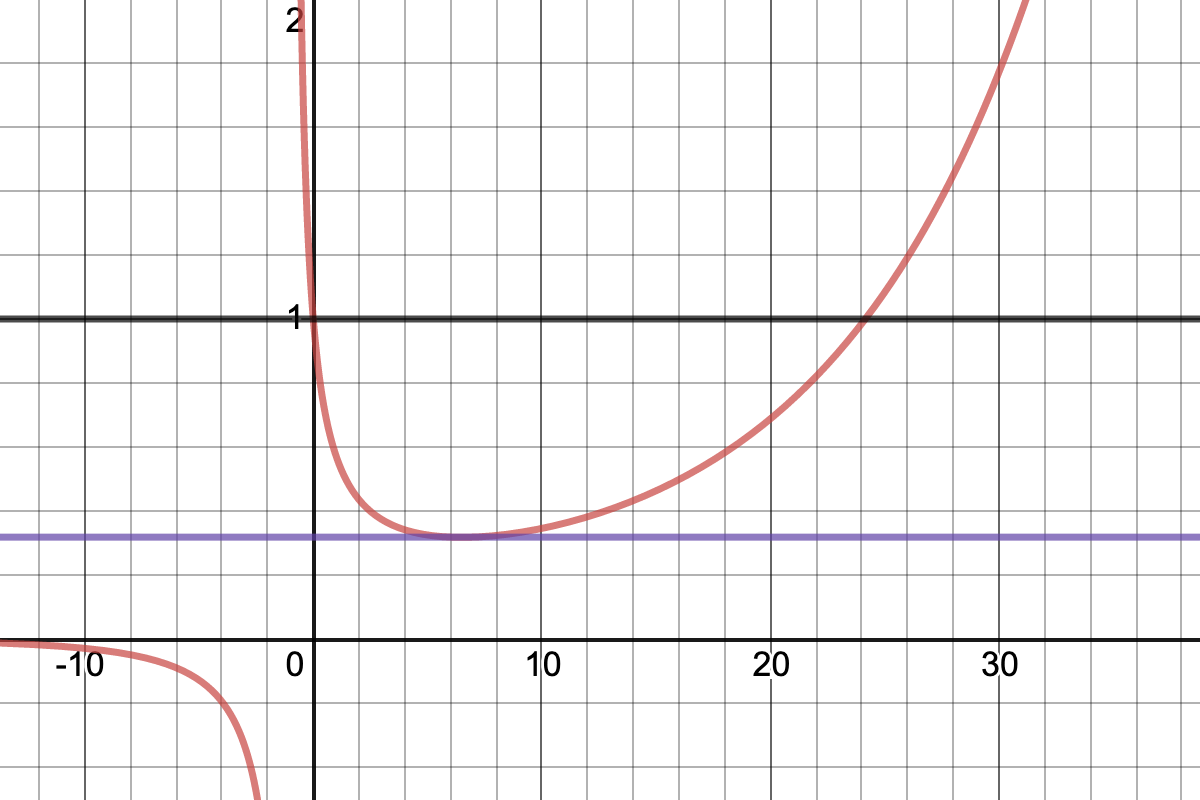
\includegraphics[scale=.2]{graphics/2.5.3.png}}
        \caption{The red line is $y=8^2/(7^2(q+1))$,
        the black line is $y=1$,
        and the purple line is $y=8^2/(7^2(6+1))$
        which is the minimum value Markov's
        inequality gives us for any moment.}
        \label{fig:2.5.3}
    \end{figure}
    \autoref{fig:2.5.3} visualizes the bound
    Markov's Inequality applied to $X^q$ gives.
    The bound gets tighter until $q=6$
    and then looser and becomes vacuous around $q=25$.

    \item
    Define $g(x)$ for $x \in [0,1]$ such that
    $g(x)=0$ if $x<7/8$ and $g(x)=1$ otherwise.
    Then $\E[g(X)] = 0 (7/8) + 1 (1/8) = 1/8$.
    Observe that $g(7/8) = 1$.
    Markov's Inequality gives
    \begin{align}
        \Pr(g(X) \geq g(\frac{7}{8})) =
        \Pr(g(X) \geq 1) \leq E[g(X)] = \frac{1}{8}.
        \nonumber
    \end{align}

\end{enumerate}


\homework{3}{R. Teal Witter}
% chktex-file 46
% chktex-file 3

\section*{Problem 1}
\textbf{Collaborators:} None.
\medskip

\begin{enumerate}
    \item Using the gradient descent algorithm
    we analyzed in class and rearranging as described in
    the problem set up, we can get a vector $y^{(i)}$
    such that
    \begin{align}
        y^{(i)} - y^* = (I - \frac{1}{\lambda_1}A^T A) (y^{(0)}-y^*)
        \nonumber
    \end{align}
    in $O(ndi)$ time.
    In order to get the desired $x^{(q)}$, we sum
    with the proper coefficients for the polynomial we want:
    \begin{align}
        x^{(q)}-x^* &=
        c_0(y^{(0)}-y^*) + c_1(y^{(1)}-y^*) + \cdots +
        c_q(y^{(q)}-y^*) \nonumber \\
        &=\left[ c_0(I) + c_1 (I - \frac{1}{\lambda_1}A^T A)
        + \cdots + c_q (I - \frac{1}{\lambda_1}A^T A)^q
        \right ] (y^{(0)}-y^*) \nonumber \\
        &=p(I- \frac{1}{\lambda_1}A^T A)(x^{(0)}-x^*).
        \nonumber
    \end{align}
    Notice that the initial starting vector $x^{(0)}=y^{(0)}$
    and that the problem doesn't change so the optimal solution
    $x^*=y^*$.
    Thus we can substitute $(x^{(0)}-x^*)$ for $(y^{(0)}-y^*)$
    between the second and third lines.
    If we save each $y^{(i)}$ as we go and use it for the $i+1$th
    iteration, we can calculate our $x^{(q)}$ in total
    time $O(ndq)$.

    \item Choose $\gamma = \lambda_d/\lambda_1$.
    By Claim 4 in the Lanczos notes,
    there is a degree $q=O(\sqrt{1/\gamma}\log(1/\epsilon))$
    polynomial $p$ such that $p(1)=1$ and $|p(t)|\leq\epsilon$
    for $0\leq t \leq 1-\gamma$.

    We check that such a $p$ is the one we want.
    Indeed, $p(1)=1$ tells us the coefficents sum to 1 which is
    exactly what we want.
    
    The eigenvalues of $A^T A$ are $\lambda_1,\ldots,\lambda_d$
    so the eigenvalues of $1/\lambda_1 A^T A$ are
    $\lambda_1/\lambda_1, \ldots, \lambda_d/\lambda_1$
    and the eigenvalues of $M=I-1/\lambda_1 A^T A$ are 
    $1-\lambda_1/\lambda_1, \ldots, 1-\lambda_d/\lambda_1$.

    Then the eigenvalues of $p(M)$ are
    $p(1-\lambda_1/\lambda_1), \ldots, p(1-\lambda_d/\lambda_1)$.
    To see this, observe that the $i$th term of $M$ for
    $0\leq i \leq q$ is $c_i M^i = c_i V\Lambda^i V^T$ where
    $M = V \Lambda V^T$.
    So the $j$th eigenvalue of $M$ is
    $p(1-\lambda_j/\lambda_1)$.

    The smallest eigenvalue is $p(1-\lambda_1/\lambda_1)=p(0)$.
    The top eigenvalue of $M$ is $p(1-\lambda_d/\lambda_1)$
    since $\lambda_d \leq \lambda_j$ for all other eigenvalues
    $\lambda_j$ of $A^T A$.
    Sure enough $p(1-\lambda_d/\lambda_1) = p(1-\gamma) \leq \epsilon$.
    This $p$ is the one we want!

    \item 
    In $q=O(\sqrt{\lambda_1/\lambda_d}\log(1/\epsilon))$
    iterations of matrix multiplication, we can get a matrix
    $p(I-1/\lambda_1 A^T A)$ with top eigenvalue bounded above
    by $\epsilon$.
\end{enumerate}

\newpage
\section*{Problem 2}
\textbf{Collaborators:} Kelly Marshall.
\medskip

\begin{enumerate}
    \item Define $f(x) = \tilde{\lambda} x^T x - x^T A^T A x$.
    We want to show that $f(x)$ is a convex function.
    Let $x,y \in \R^d$ and $s \in [0,1]$.
    Then
    \begin{align}
        (1-s)f(x)+sf(y) &= (1-s)\tilde{\lambda} x^T x - (1-s)x^T A^T A x
        + s\tilde{\lambda} y^T y - sy^T A^T A y \nonumber \\
        \label{eq:convexmid}
        &\geq (1-s)^2\tilde{\lambda} x^T x - (1-s)^2x^T A^T A x
        + s^2\tilde{\lambda} y^T y - s^2y^T A^T A y
    \end{align}
    since $0 \leq s \leq 1$ and $f(x) \geq 0$ imply that
    $(1-s)f(x) \geq (1-s)^2f(x)$ and $sf(y) \geq s^2f(y)$.
    Notice that $f(x) \geq 0$ follows from the supposition
    that $v_1$ is the $\arg \min$ of $f(x)$
    since $v_1 A^T A v_1 = \lambda_1 \leq \tilde{\lambda}$
    by assumption.
    Continuing from \autoref{eq:convexmid},
    \begin{align}
        &= \tilde{\lambda} (1-s) x^T (1-s) x - (1-s)x^T A^T A (1-s)x
        + \tilde{\lambda} s y^T s y - sy^T A^T A sy
        &=f((1-s)x + s y)
        \nonumber
    \end{align}
    by linearity.
    Therefore $f(x)$ is convex.

    To see that $S$ is not convex,
    choose vectors $e_1$ and $e_2$ and scalar $1/2$.
    Both $\norm{e_1}^2 = \norm{e_2}^2=1$ so
    $e_1, e_2 \in S$ but
    $\norm{1/2 e_1 +1/2 e_2}^2 = 1/4 + 1/4 = 1/2 < 1$
    so the linear combination $1/2 e_1 +1/2 e_2 \notin S$.

    \item To show that projected gradient descent
    with $f(x)$ and $S$ is exactly equivalent to
    the power method, we need to show that the update
    rules are the same and the final vector
    in the power method is the $\arg \min$
    over all the vectors.

    We can write
    \begin{align}
        f(x) = \tilde{\lambda}\sum_{i=1}^n x_i^2 
        - \sum_{i=1}^n \left(\sum_{j=1}^d a_{i,j} x_j \right)^2
        \nonumber
    \end{align}
    where $a_{i,}$ is the $i$th row of $A$.
    Then
    \begin{align}
        \frac{\partial f}{\partial x_j}
        &= 2 \tilde{\lambda} x_j - \sum_{i=1} 2a_{i,j} (a_{i,} \cdot x)
        = 2 \tilde{\lambda} x_j - 2a_{,j}^T (A x)
        \nonumber \\
        \label{eq:gradient}
        \nabla f(x) &=
        2 \tilde{\lambda} x - 2 A^T A x.
    \end{align}
    For $x{(i)} - \eta \nabla f(x^{(i)}) = A^T (A z^{(i)})$,
    we choose $\eta = 1/(2\tilde{\lambda})$.

    To see that the projection step is the same as normalizing,
    simply recall that $S$ is the set of vectors with 
    norm greater than or equal to 1.

    The $\arg \min$ returned by projected gradient descent
    is the same as the final vector $z^{(T)}$ from the 
    analysis in class that each $z$ moves closer and closer
    to $v_1$.

    \item
    Define $g(x) = -(x^T A^T A x)/ (x^T x)$.
    Then 
    \begin{align}
        \nabla g(x) &= 
        - \frac{x^Tx2A^TAx - x^T A^T A x 2x}{(x^Tx)^2}
        \nonumber \\ &=
        \frac{2}{(x^Tx)^2}\left( x^TA^TAx x - x^T x A^T A x\right).
        \nonumber
    \end{align}

    For any scaling $c$ and right singular vector
    $v_i$,
    $c v_i^TA^T A c v_i = c^2 \sigma_i^2$
    and $A^T A v_i = c \sigma_i^2 v_i$.
    Therefore $c^3 v_i^T A^T A v_i v_i = c^2 \sigma_i^2 c v_i
    = c^3 v_i^T v A^T A v_i$
    so $\nabla g(c v_i)=0$ and $cv_i$ must be a stationary point.
    
    To see that $g$ is non-convex, choose vectors $v_d$ and $v_1$.
    Then
    \begin{align}
        g(v_d) - g(v_1) = -\sigma_d^2 + \sigma_1^2  > 0
        = \nabla g(v_d)^T (v_d - v_1) \nonumber
    \end{align}
    so $g$ is not convex.

    \item
    Choose $z= v_1$.
    Then
    \begin{align}
        g(v_i + tv_1) = -\frac{(v_i+tv_1)^TA^TA(v_i+tv_1)}
        {\norm{v_i + tv_1}^2} = 
        \frac{-\sigma_i^2 - t\sigma_1^2}
        {1+t}
        \nonumber
    \end{align}
    because of the orthonormal
    property of $v_i$ and $v_1$.
    Since $\sigma_1 > \cdots > \sigma_d$ by assumption,
    \begin{align}
        g(v_i + tv_1) = 
        \frac{-\sigma_i^2 - t\sigma_1^2}{1+t}
        < \frac{-\sigma_i^2 - t\sigma_i^2}{1+t}
        = g(v_i).
        \nonumber
    \end{align}

\end{enumerate}

\newpage
\section*{Problem 3}
\textbf{Collaborators:} Indu Ramesh.
\medskip

\begin{enumerate}
    \item We sum the rows and columns of $D$.
    First observe that
    \begin{align}
        D_{i,j} &= \norm{x_i - x_j}^2 \nonumber \\
        &= (x_i - x_j)^T (x_i - x_j) \nonumber \\
        &= \norm{x_i}^2 + \norm{x_j}^2 - 2 x_j^T x_i \nonumber.
    \end{align}
    Then
    \begin{align}
        \sum_{j=1}^n \sum_{i=1}^n D_{i,j} &=
        \sum_{j=1}^n \sum_{i=1}^n \norm{x_i}^2 + \norm{x_j}^2
        - 2x_j^T x_i \nonumber \\
        &= \sum_{j=1}^n \sum_{i=1}^n \norm{x_i}^2 +
        \sum_{i=1}^n \sum_{j=1}^n \norm{x_j}^2 +
        \sum_{j=1}^n -2 x_j^T \sum_{i=1}^n x_i \nonumber \\
        &= 2n \sum_{i=1}^n \norm{x_i}^2
        \nonumber
    \end{align}
    where we use the assumption that $\sum_{i=1}^n x_i$
    is the all 0s vector.
    Therefore $\sum_{i=1}^n \norm{x_i}^2 = ||D||_F^2 / (2n)$.
    We simply iterate and sum over $D$ in time $O(n^2)$ where
    $D$ is $n\times n$.

    \item 
    We begin by summing each row
    \begin{align}
        \norm{D_{i,}}^2 &= \sum_{j=1}^n \norm{x_i}^2 + \norm{x_j}^2
        - 2 x_i^T x_j \nonumber \\
        &= n \norm{x_i}^2 + \sum_{j=1}^n \norm{x_j}^2 - 0.
        \nonumber
    \end{align}
    Then the difference of the sums of two rows yields
    \begin{align}
        \norm{D_{i,}}^2 - \norm{D_{k,}}^2 &= 
        n (\norm{x_i}^2 - \norm{x_k}^2).
        \nonumber
    \end{align}
    Fix $i$. We sum
    \begin{align}
        \sum_{k=1}^n D_{i,k} + \frac{\norm{D_{i,}}^2 - \norm{D_{k,}}^2}{n}
        &= \sum_{k=1}^n 2 \norm{x_i}^2 - 2 x_{i}^Tx_k \nonumber \\
        &= 2n \norm{x_i}^2 - 0.
        \nonumber
    \end{align} 
    Therefore
    \begin{align}
        \frac{1}{2n}
        \sum_{k=1}^n D_{i,k} + \frac{\norm{D_{i,}}^2 - \norm{D_{k,}}^2}{n}
        = \norm{x_i}^2.
        \nonumber
    \end{align}
    We calculate each $\norm{D_{i,}}^2$ in time $n$
    then the summation over $k$ adds another factor of $n$.
    Therefore we can calculate $\norm{x_i}^2$ in $O(n^2)$ time.

    \item We define a $n \times n$ matrix $G$ where entry
    $G_{i,j} = x_i^T x_j$.
    With the set of $\norm{x_i}^2$ terms from the previous problem,
    we can calculate $x_i^T x_j = (\norm{x_i}^2 + \norm{x_j}^2 - D_{i,j})/2$
    in constant time.
    So in an additional $O(n^2)$ time we can contruct the matrix $G$.

    Clearly $G = X^T X$ where $X$ is the $d \times n$ matrix whose columns
    are the vectors $x_i$ for $i \in [n]$.
    Then $G$ is positive semi-definite and we can find $X$ either by
    performing an eigenvalue decomposition or singular value decomposition.
    The time complexity for both operations is an additional $O(n^3)$.
\end{enumerate}




	
	
\end{document}